\documentclass[tikz,border=4pt]{standalone}
% Estilo común de los diagramas de bloques (se usa con \input en cada standalone)
\usepackage[defaultsans,scale=0.92]{lato}
\usepackage{libertinust1math}
\usepackage{xcolor,amsmath}
\usepackage{tikz}
\usetikzlibrary{positioning,arrows.meta,calc,shapes.geometric}
\usepackage{../../notacion}
\definecolor{ctrlazul}{HTML}{1E5AA8}\definecolor{ctrlnoche}{HTML}{14213D}
\definecolor{ctrlcoral}{HTML}{D1495B}\definecolor{ctrlverde}{HTML}{2A9D8F}
\definecolor{ctrlambar}{HTML}{E09F3E}\definecolor{ctrlgris}{HTML}{5C677D}
\definecolor{ctrlvioleta}{HTML}{6C4AB6}\definecolor{ctrlteal}{HTML}{0F7173}
\tikzset{
  >={Stealth[length=2.4mm]}, every node/.style={font=\small},
  bloque/.style={draw=ctrlnoche,fill=ctrlazul!7,thick,rounded corners=1.5pt,minimum height=9mm,minimum width=13mm,inner sep=4pt},
  suma/.style={draw=ctrlnoche,thick,circle,inner sep=0pt,minimum size=6mm},
  senal/.style={->,thick,draw=ctrlnoche},
  rot/.style={font=\footnotesize,text=ctrlgris},
}

\begin{document}
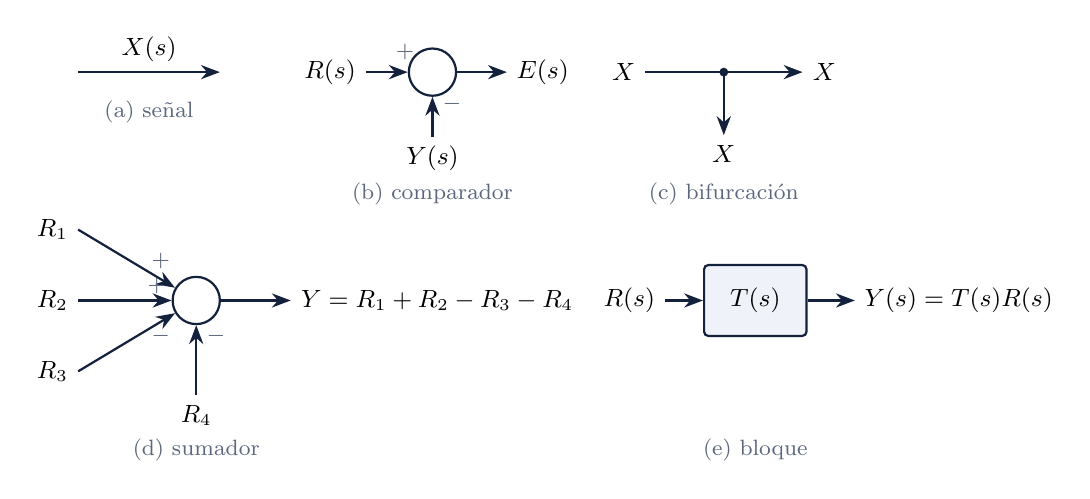
\begin{tikzpicture}[node distance=8mm]
  % a) señal
  \draw[senal] (0,0)--node[above]{$X(s)$}(1.8,0); \node[rot] at (0.9,-0.5) {(a) señal};
  % b) comparador
  \begin{scope}[xshift=3.2cm]
    \node (r) at (0,0) {$R(s)$}; \node[suma] (S) at (1.3,0) {}; \node (e) at (2.7,0) {$E(s)$};
    \node (yb) at (1.3,-1.1) {$Y(s)$};
    \draw[senal] (r)--(S); \draw[senal] (S)--(e); \draw[senal] (yb)--(S);
    \node[rot] at (0.95,0.25) {$+$}; \node[rot] at (1.55,-0.4) {$-$};
    \node[rot] at (1.3,-1.55) {(b) comparador};
  \end{scope}
  % c) bifurcación
  \begin{scope}[xshift=7.2cm]
    \draw[senal] (0,0)--(2,0) node[right]{$X$}; \fill[ctrlnoche] (1,0) circle (1.6pt);
    \draw[senal] (1,0)--(1,-0.8) node[below]{$X$}; \node[left] at (0,0) {$X$};
    \node[rot] at (1,-1.55) {(c) bifurcación};
  \end{scope}
  % d) sumador múltiple
  \begin{scope}[yshift=-2.9cm]
    \node[suma] (S2) at (1.5,0) {};
    \draw[senal] (0,0.9) node[left]{$R_1$}--(S2); \draw[senal] (0,0) node[left]{$R_2$}--(S2);
    \draw[senal] (0,-0.9) node[left]{$R_3$}--(S2); \draw[senal] (1.5,-1.2) node[below]{$R_4$}--(S2);
    \node[rot] at (1.05,0.5) {$+$}; \node[rot] at (1.0,0.18) {$+$}; \node[rot] at (1.05,-0.45) {$-$}; \node[rot] at (1.75,-0.45) {$-$};
    \draw[senal] (S2)--(2.7,0) node[right]{$Y=R_1+R_2-R_3-R_4$};
    \node[rot] at (1.5,-1.9) {(d) sumador};
  \end{scope}
  % e) bloque
  \begin{scope}[xshift=7.0cm,yshift=-2.9cm]
    \node (x) at (0,0) {$R(s)$}; \node[bloque] (T) at (1.6,0) {$T(s)$};
    \node[right=6mm of T] (y) {$Y(s)=T(s)R(s)$};
    \draw[senal] (x)--(T); \draw[senal] (T)--(y);
    \node[rot] at (1.6,-1.9) {(e) bloque};
  \end{scope}
\end{tikzpicture}
\end{document}
